\documentclass[crop,tikz,convert=pdf2svg]{standalone}
%\usetikzlibrary{...}% tikz package already loaded by 'tikz' option
\usetikzlibrary{calc}
\usepackage{ latexsym }
\begin{document}
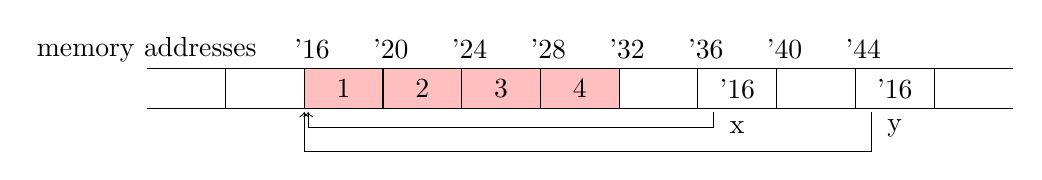
\begin{tikzpicture}% Example:

\draw[fill=red!25] (2,0) -- (6,0) rectangle (2, 0.5) -- (6, 0.5);
\draw (0,0) -- (11,0);
\draw (0,0.5) -- (11,0.5);
\foreach \i in {1,...,10}
    \draw (\i, 0) -- (\i, 0.5);
\node at (0, 0.75) {memory addresses};
\foreach \i in {16,20,24,28,32,36,40,44}
    \node at (\i/4-2+0.1, 0.75) {'\i};
\foreach \i in {1,...,4}
    \node at (\i+1.5, 0.25) {\i};
\node at (7.5, -0.25) {x};
\node at (7.5, 0.25) {'16};
\draw[->] (7.2, -0.05) -- (7.2, -0.25) -- (2.05, -0.25) -- (2.05, -0.05);
\node at (9.5, -0.25) {y};
\node at (9.5, 0.25) {'16};
\draw[->] (9.2, -0.05) -- (9.2, -0.55) -- (2.0, -0.55) -- (2.0, -0.05);

\end{tikzpicture}
\end{document}
